\begin{figure}[tb]
  \centering
  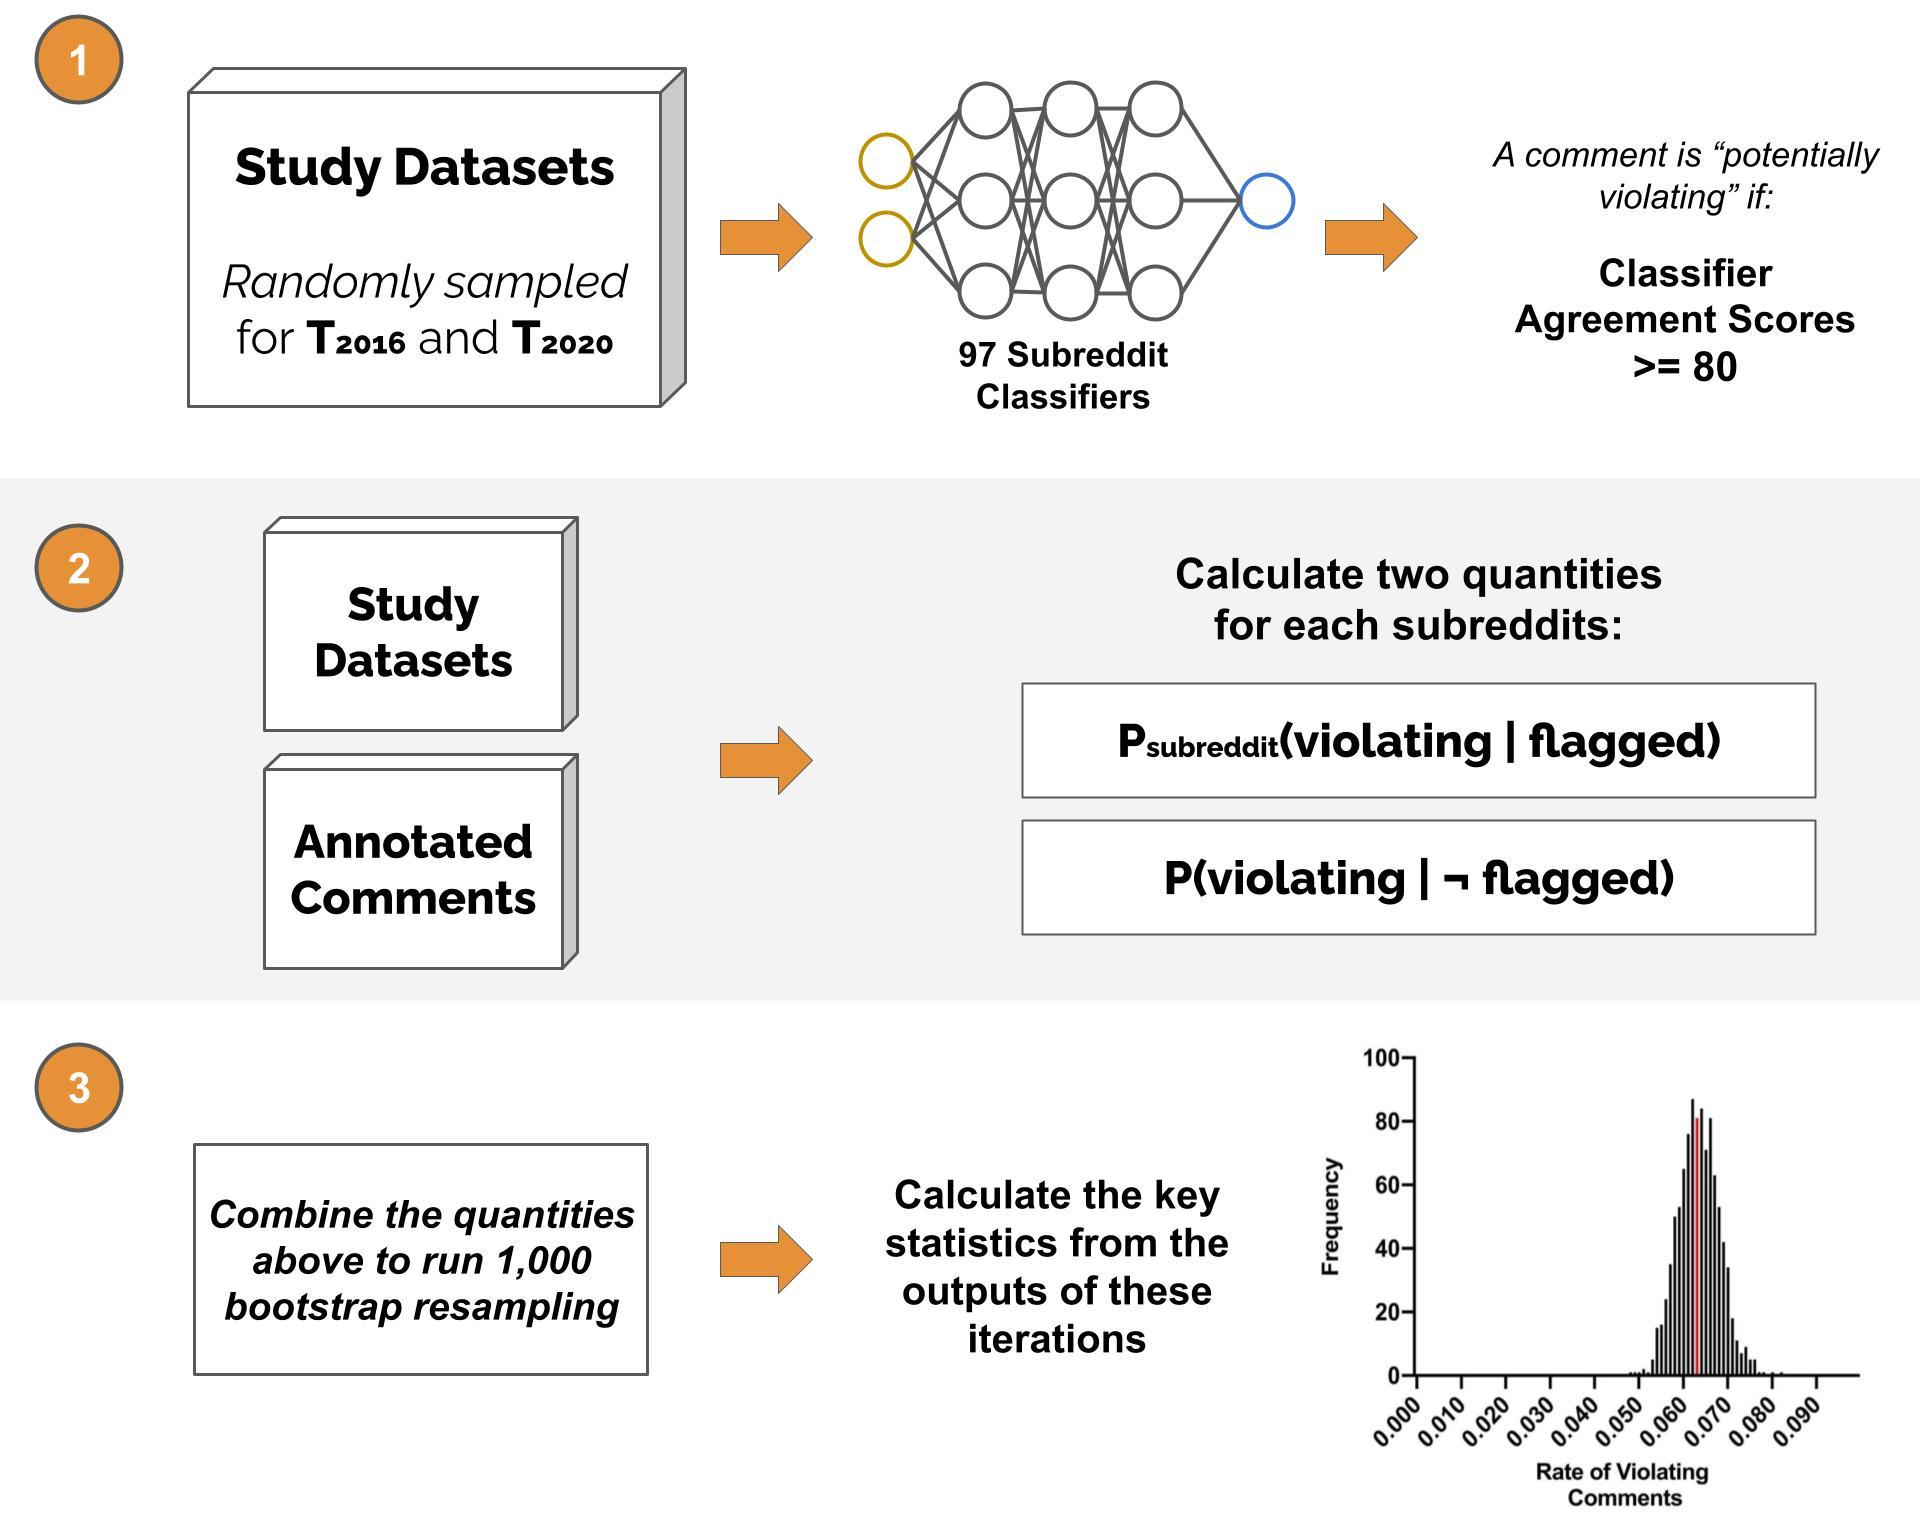
\includegraphics[width=1.0\textwidth]{content_minor_revision__Apr2022/images/bootstrap_workflow_6.jpg}
  \caption{\rnr{An overview of the sampling process in broad strokes. We start by randomly sampling unmoderated comments from $T_{2016}$ and $T_{2020}$ to generate our study datasets. We then use these datasets and the annotated comments to calculate key quantities that are needed for our bootstrap resampling. We then combine these quantities to implement our resampling procedure, which we repeat 1,000 times for each time periods of our interest.}}
  \label{fig:bootstrap}
  \Description{Bootstrap resampling workflow}
\end{figure}